
%BETTER TITLE
%TEAM NAME
%PROJECT NAME

%write a paragraph on the scripting langauage
%make gantt chart
\documentclass[a4paper,12pt]{article}

\addtolength{\oddsidemargin}{-.5in}
\addtolength{\evensidemargin}{-.5in}
\addtolength{\textwidth}{1in}
\addtolength{\topmargin}{-.875in}
\addtolength{\textheight}{1.75in}

\usepackage{graphicx}
\usepackage{multicol}
\usepackage{listings}
\lstset{language=Python} 

\begin{document}

%\\*Project Proposal
%\\*Prepared for: Andrew Trotman, Lecturer
%\\*Prepared by: The Famous Five
%\\*4 April 2014
%\\*Proposal Name: Five Make a Unicorn Shell

%\title{Project Proposal}
%\author{Richie, Chris, Tom, Shaun, Reuben}
%\date{\today}


\begin{titlepage}

  \newcommand{\HRule}{\rule{\linewidth}{0.5mm}}
  \center
  \textsc{\LARGE COSC345 Assignment 1}\\[0.5cm] 
  \textsc{\Large Project Proposal}\\[0.5cm] 
  %\textsc{\large COSC345 Assignment 1}\\[0.5cm]

  \HRule \\[0.6cm]
         { \huge \bfseries Unicorn Shell}\\[0.4cm]
         \HRule \\[1.5cm]
         
         \Large \emph{Prepared by:}\\
         \begin{multicols}{3}
           Richie \textsc{McKee}\\
           Shaun \textsc{Wratten}\\
           \columnbreak
           Chris \textsc{McMillan}\\
           Thomas \textsc{Hall}\\
           \columnbreak
           Reuben \textsc{Crimp}\\[3cm]
         \end{multicols}
         
         \null\vfill{\large \today}\\[3cm]
\end{titlepage}

\section*{Introduction}
Thank you for choosing to read our project proposal

We are extremely excited to show you our proposal. When set with the task of designing and creating a new shell we had a number of ideas that sprang to mind and a great deal more that became more apparent to us as we researched shells in greater detail and found things that we felt a shell would benefit from having.

%\section*{Project Description}
We want a shell that has all the features of popular shells like the Bourne Again Shell. However we will attempt to add features that make it far more usable and also include additional features that make our shell standout, encouraging people to adopt our obviously superior piece of software.

\section*{Project Overview}

The Unicorn Shell (working title) will be a modern, POSIX style shell which will be released on linux, OSX and Windows under the FreeBSD License. The project will written almost entirely in C++ and al the source code will be released in it's entirety.

The Unicorn Shell will be targeted at those of beginner level, people who are not particularly skilled at using a shell, and possibly even those who have never used one before.

The shell will be developed to be intuitive. Basic shell operations will be natural interactions, that most computer users are familiar with, anyone will be able to pickup unicorn very quickly, even those from different OS backgrounds.

Despite the target audience of our Shell, it will still provide the full feature set that advanced users would expect.

Such features will include tab-completion, inline command prediction and detection, stream redirection, job control,  command history and aliases. And almost everything will be able to be customised.

It will also look pretty with proportional width font, no more ugly mono-spaced garbage, only beautifully kerned Helvetica. 

\pagebreak
\section*{The Team}

\subsection*{Reuben Crimp (Surgeon):}
Reuben began programming in high school, making what interested him: games and websites. He graduated highschool in 2011 doing well in mathematics. He enrolled at Otago University in mid 2012, with computer science as a major, mathematics for a minor. He has very little industry experience but a strong passion for the subject matter.

\subsection*{Shaun Wratten (Co-pilot):}
Shaun recently graduated from UCOL in Palmerston North with a Bachelor’s degree in Information and Communications Technology,
%in which he learnt a decent portion of his skill set. This includes programming in
has has experience with
C\#, C++, scripting and web design using PHP and JavaScript, and working with MS-SQL and MySQL database. One of the major things he learned while studying was how to
%strutter ??
strutter a team project and how to be as successful leader and team member.

\subsection*{Chris McMillan (Toolsmith):}
Chris has studied at the University of Otago since 2010, but only became interest in computers after high school. He completed a chemistry degree and then decided that his passion lay in computers and began study towards a computer science major as well. He will finish his BSc double major at the end of 2014. His main strengths are music and audiosoftware. Chris can confidently write in both Java and Python, but building a shell in C++ will be a challenge for him that he looks forward to and hopes to learn a lot from.

\subsection*{Thomas Hall (Language Guru and Tester):}
Thomas is a recent graduate with BSc in Physics. He is currently studying a DipGrad in computer science to be finished in early 2015. He has experience programming in C\# from experimenting with Unity, and Matlab as part of his physics education. He also has a experience with Java and Python.

\subsection*{Richie McKee (Editor and Program Clerk):}
Richie completed his LLB/BA at the end of 2012 at Otago University. He always had a strong desire to learn computer science but is only now taking steps towards doing so. He began his DipGrad at the start of 2014 and hopes to be completed by the end of the year. As such his current level of experience is limited and his experience with programming is limited to what he learned during Summer School and what he is currently covering throughout the semester. To him the project is a daunting but exciting prospect that he hopes to learn from.

\pagebreak
\section*{Tools and Hardware}

Our development enviroment will be the lab machines with OSX and GNU/linux.
Our windows dev enviroment will be our own private windows 7 64-bit machine.
\subsection*{Development tools}
\begin{multicols}{3}
  \subsubsection*{Windows}
    Visual Studio 2013 \\
    C++ libraries \\
    WIN32 \columnbreak
  \subsubsection*{OSX}
    Xcode \\
    C++ libraries \\
    Cocoa graphics \columnbreak
  \subsubsection*{GNU/Linux}
    vim, g++ \\
    C++ libraries \\
    X11
\end{multicols}
\subsection*{Revision Control}
We will use git for our distributed revision control, with project hosting by github.com.
\section*{The Shell}
As mention earlier, this shell will be released on linux, OSX and windows, and will come with most of the features you'd expect from a modern shell. as well as several usability enhancements described in the sections below.
\begin{multicols}{4}
\noindent
Stream redirection \\
Piping \\
Tab completion \\
Command history \\
Job control \\
Aliases \\
Directory stack
\end{multicols}
\subsection*{Modularised Code}

The diagram below shows the modules we plan to implement, but more importantly how input gets handled and processed.

\begin{center}
  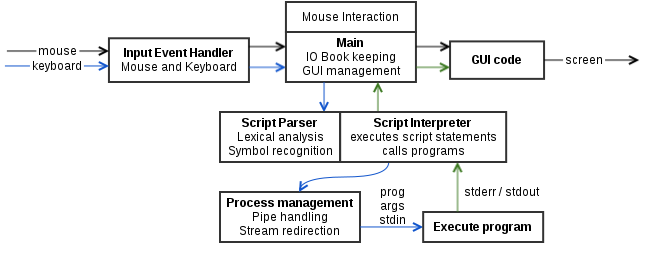
\includegraphics[width=16cm]{shellflow.png}\\
  \small Fig 0 - Flow of information through our shell
\end{center}

\pagebreak
%\subsection{Cross OS file support}
%Different operating systems by convention define a new line within a file differently
%We will allow the user to choose how to handle cross platform files

%\begin{tabular}{l | l}
%Fix & edit as current OS, save as current OS (Forced when parsing a script) \\
%Compatibility & edit as current OS, save as original. \\
%Do nothing & edit as original save as original. \\
%Custom & Fix; but you can specify the replacement terminator \\
%{‘\textbackslash r’, ‘\textbackslash n’, ‘\textbackslash r \textbackslash n’, ‘\textbackslash n \textbackslash r’}
%\end{tabular}

\subsection*{Usability Features}
The shell will allow for intuitive mouse interactions, these interactions will be very similar to the actions in a standard GUI OS environment (i.e. double click for open).

However, most of our actions wont actually perform the action outright, instead it will paste the command that would perform the requested action into the current prompt, i.e. clicking "delete file" in a *nix environment will paste the command "rm \textless file-name\textgreater" into the prompt, the user will then have to press "return" to execute the command.

The purpose of this is to help the user if they do not know the specific text command, and then to teach that particular command to them.

\begin{center}
  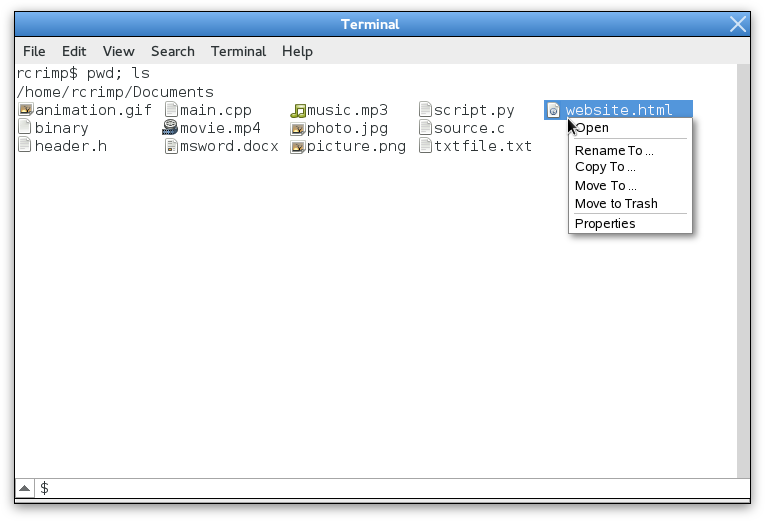
\includegraphics[width=13cm]{context2.png}\\
  \small Fig 1 - Graphical ls with context menu
\end{center}
\subsection*{Intuitive directory navigation}
Our shell will come with an inbuilt 'ls' function, designed specifically to aid beginners
(which is replaceable with the OS default ls/dir)\\*
File-names will be preceded by a filetype icon, like a GUI shell, see (fig.1)\\

Clicking on a directory will paste the command "cd \textless dir-name\textgreater" into the prompt.\\*
Double clicking a directory will execute the command "cd \textless dir-name\textgreater".\\*
Right clicking on a directory will open a context menu (see fig.1), which will list basic directory commands e.g "open (cd)", "move to .. (mv), clicking on these will paste the corresponding command into the prompt.
\subsection*{Intuitive file interaction}
Single, double and right clicking on a file, will exhibit similar results to clicking on a directory.
Single clicking on a file will paste the ``\textless file-name\textgreater'' into the current prompt.
Double clicking on a file will open the file with the OS default application (if one exists).

Right clicking a file will also  open a context menu with similar commands listed (move, rename, delete, open etc....)

\begin{center}
  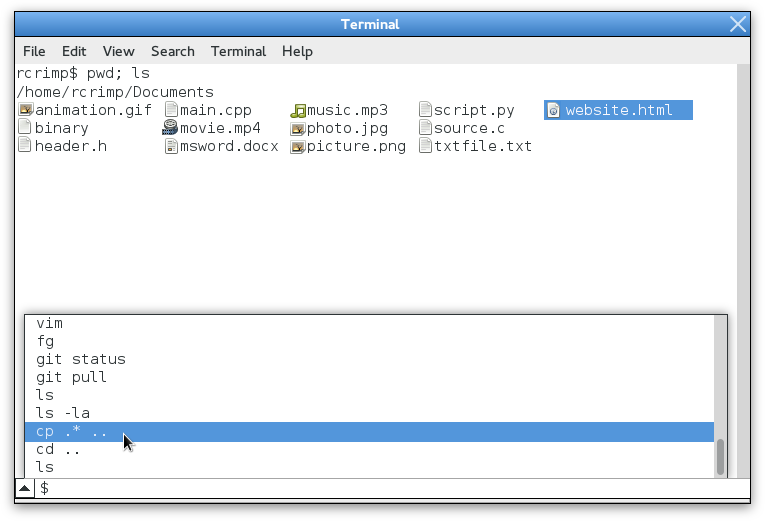
\includegraphics[width=13cm]{history2.png}\\
  \small Fig 2 - Interactive history
\end{center}

\subsection*{Interactive viewing of the command history}
clicking the small arrow to the left of the prompt, will open a drop down menu (upwards), showing the last commands executed in ascending order, allowing for easy access

The standard bash style keyboard shortcuts to access your history will also exist for the
more advanced user. (up, down, "!!", ``!str" etc...)

\subsection*{Directory Bookmarks}
We will allow users to set directory bookmarks with a quick command.

Executing ``set \#work'' will set a bookmark in the current directory called "work", then executing ``\#work'' will change the users directory back to directory in which it was set.\\*
So quick navigation between commonly accessed directories when working on a project.\\[0.5cm]
We will also implement a directory stack, for the more technically savvy user.\\*
``\#back'' and ``\#forward'' will be reserved for intuitive interaction with  directory stack, which will match the ``back'' and ``forward'' buttons on the toolbar.


\pagebreak
\subsection*{Tab Completion}

Pressing the tab key will attempt to complete the current unfinished symbol written in the prompt, i.e tabbing on ``rmdir Docu'' will try and complete the ``Docu'' symbol.\\
For example: ``Documents'', if such a directory exists.

The completions for a symbol will be dependent on the current content of the symbol and what the shell is expecting, e.g. if the shell expects the current symbol to be a file, then the shell will only search for files.

\subsubsection*{Tab-tab}
If there are multiple possible completions for the current symbol we write all of these completions to the console, letting the user view their choices.

After writing all completions for the current symbol, successive tabbing  won't redundantly list them out again (like BASH), instead we will cycle through the possible completions inline in the prompt.  

\subsubsection*{Wild card}
Our shell will treat a '*' in the prompt as a ``wild card'', i.e * will lazily match any string, even the empty string. \\
so ``*.c'' would match ``source.c'', ``main.c'' and even ``.c''

\subsubsection*{Parent directories}

The parent directories of the working directory will be included when completing a directory name, so navigating back up a file structure is easier.

No longer will you need to ``cd ../../../../''

\subsection*{If we have time}
More rigorous pattern recognition, using wildcards can be very powerful, but more fine grained filtering would be nice - maybe.\\[0.5cm]
A tab complete function for man pages, i.e ``man 3 *fpr'' would complete the last symbol as ``printf'',  ``fprintf'' ...\\[0.5cm]
Real time inline command prediction.

\pagebreak
\section*{Script Syntax}

We will use end statements and colons to delimit program blocks.

\begin{multicols}{2}

  \subsubsection*{Keywords}
  \begin{tabular}{| l | l | l | l | } \hline
    and & fail & if & return \\ \hline
    break & false & in & true \\ \hline
    class & for & not & try \\ \hline
    else & function & or & unicorn \\ \hline
    end & global &  print & while \\ \hline
  \end{tabular}

  \subsubsection*{Arithmetic operators}
  \begin{tabular}{| l | l | } \hline
    + & Addition \\ \hline
    - & Subtraction \\ \hline
    * & Multiplication \\ \hline
    \textbackslash & Division \\ \hline
    \% & Modulus \\ \hline
    \(\wedge\)  & Exponent \\ \hline
  \end{tabular}

  \subsubsection*{Assignment operators}
  \begin{tabular}{| l | l | } \hline
    = & Simple assignment  \\ \hline
    += & Add and assignment  \\ \hline
    -= & Subtract and assignment  \\ \hline
  \end{tabular}

  \subsubsection*{Comparison Operators}
  \begin{tabular}{| l | l | } \hline
    == & Equal \\ \hline
    != & Not equal \\ \hline
    \textgreater & Left larger \\ \hline
    \textless & Right Larger \\ \hline
    \textgreater= & Left larger than or equal to \\ \hline
    \textless= & Right larger than or equal to \\ \hline
  \end{tabular}

\end{multicols}

\subsection*{Code Examples}
\begin{multicols}{2}
  \subsubsection*{foo function in C}
  \begin{lstlisting}
    void foo(int x) {
      if (x == 0) {
        bar();
        baz();
      } else {
        quz(x);
        foo(x - 1);
      }
    }
  \end{lstlisting}
  \subsubsection*{foo function in unicorn}
  \begin{lstlisting}
    function foo(x):
    if x == 0:
    bar()
    baz()
    else:
    qux(x)
    foo(x - 1)
    end
    end
  \end{lstlisting}
\end{multicols}

\pagebreak
\section*{Risk Analysis}

We wanted to implement a proactive approach to dealing with risks as opposed to a reactive approach.

Our objective is to be able to avoid risk whenever possible, and to solve problems before they manifested themselves. This preparation would hopefully mean that we could respond to problems that did occur in a controlled and effective manner. We understand that risks evolve throughout the course of the project and so we will be constantly monitoring identified risks throughout the course of the year via a risk map to ensure that we are still keeping them at bay. 

\section*{Project Schedule}

Dependencies between activities - allocation of people to tasks, time until milestones

Monitoring the project and ourselves is an important way for us to anticipate future
problems and gives us a chance to avoid them.
Sticking to the Gantt Chart, Pert Chart - make sure on schedule
reporting - GIT hub - so every time we make a build we push it.

((How it will be monitored and when will reports be delivered))
\end{document}
